%%%%%%%%%%%%%%%%%%%%%%%%%%%%%%%%%%%%%%%%%%%%%%%%%%%%%%%%%%%%%%%%%%%%%%%%
%                                                                      %
%     File: Control_methods_overview.tex                               %
%     Tex Master: Thesis.tex                                           %
%                                                                      %
%     Author: Israel Sother                                            %
%     Last modified: 27 May 2024                                       %
%                                                                      %
%%%%%%%%%%%%%%%%%%%%%%%%%%%%%%%%%%%%%%%%%%%%%%%%%%%%%%%%%%%%%%%%%%%%%%%%
\vfill
\section{Control Methods State of the Art}\label{section:control_methods}
The quest for higher efficiency and performance has pushed the development in the field of control of electrical machines, and even though several advances have been made, the main strategies in the market are still the \gls{foc} with PID current control, and \gls{dtc}. While robust and well-known, these methods cannot explore the full performance envelope of the controlled machines, and the development of more complex machines with increased dynamic response and efficiency has pushed for new control strategies. In this context, the use of \gls{mpc} has grown as a good alternative as it explicitly considers the system dynamics and constraints.

\subsection{Field Oriented Control}

For many years field oriented control has been one of the cornerstones of electrical machine control due to its simplicity and easy implementation~\cite{Doncker:Universal_FOC:1994}. This technique is based on the Blondel Park transformation, where it converts the currents and voltages from a stationary ABC reference frame into a rotating referential dq0. This allows the individual control of the motor magnetic flux and torque, which are proportional to $i_d$ and $i_q$ respectively. These currents usually are controlled using two separated PIDs, where the quadrature current reference comes from the desired motor torque and the direct current comes from the field weakening strategy. The PIDs compare the references with the measured values and output a voltage to be applied in each axis, voltages that are passed to a modulator (usually \gls{svm}) to calculate the duty cycle of each MOSFET and generate the control signals. An example of such a system is shown in \Cref{fig:example_PID}.
\begin{figure}[!htb]
	\centering
	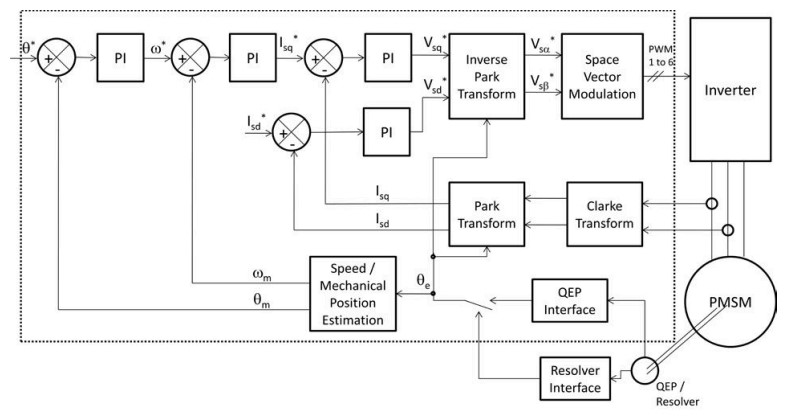
\includegraphics[width=1\textwidth]{Figures/foc_texas_instruments.jpg}
	\caption[Field Oriented Control - from Texas Instruments~\cite{TI:FOC_TMS320F2837:2016}.]{Field Oriented Control - from Texas Instruments~\cite{TI:FOC_TMS320F2837:2016}.}
	\label{fig:example_PID} %chktex 24
\end{figure}

While simple and robust, this technique heavily depends on the rotor position which is not always available, thus often needing some form of estimation to work correctly. Despite this limitation, \gls{foc} is a versatile method, being suitable not only for \gls{pmsm}, but also for induction motors, reluctance machines, among others~\cite{Hoang:FOC_vs_DTC_induction:1999,Matsuo:FOC_reluctance:1993}. One of the great advantages of \gls{foc} is that it produces a smooth operation in the full range of the motor, with low current distortions and reduced torque ripple~\cite{Adhavan:FOC_fuzzy:2011}.



\subsection{Direct Torque Control}
The principal rivel of \gls{foc} is \gls{dtc}, it shows better dynamic response with simpler implementation and less dependency on machine characterization~\cite{Hoang:FOC_vs_DTC_induction:1999}. Popularized by its use on induction machines, this method usually operates at the abc reference frame, calculating the flux based on the voltage and current vectors as in \Cref{eq:dtc_flux}, where $V_s$ is the stator voltage vector, $I_s$ is the stator current vector, $R_s$ is the stator resistance matrix, and $\psi_r$ is the rotor magnetic flux vector. Using this information, the torque can be calculated as in \Cref{eq:dtc_tq}, where $p$ is the number of pole pairs. When using an induction machine it is not necessary to have a rotor position, but on \gls{pmsm} this becomes a necessity as in \gls{foc}.

\begin{subequations}
	\begin{minipage}{.45\linewidth}
        \begin{equation}
            \psi_s = \int (V_s -R_s I_s)dt + \psi_r
            \label{eq:dtc_flux}
        \end{equation}
    \end{minipage}
    \begin{minipage}{.45\linewidth}
        \begin{equation}
            T_e = p(\psi_s I_s)
            \label{eq:dtc_tq}
        \end{equation}
    \end{minipage}
\end{subequations}

With these states calculated, a simple hysteresis band is applied to each, torque and flux, to select one of the 8 possible voltage vectors. This selection is done based on a lookup table that depending on the output of both hysteresis controllers, chooses the vector that pushes the torque and flux towards its references. This table can be generated using several strategies with different resultant dynamics~\cite{Buja:DTC_lookup_strategies:1997,Nasr:DTC_PMSM_improvement:2022}. The general schema of the \gls{dtc} is shown in \Cref{fig:example_DTC}.
\begin{figure}[!htb]
	\centering
	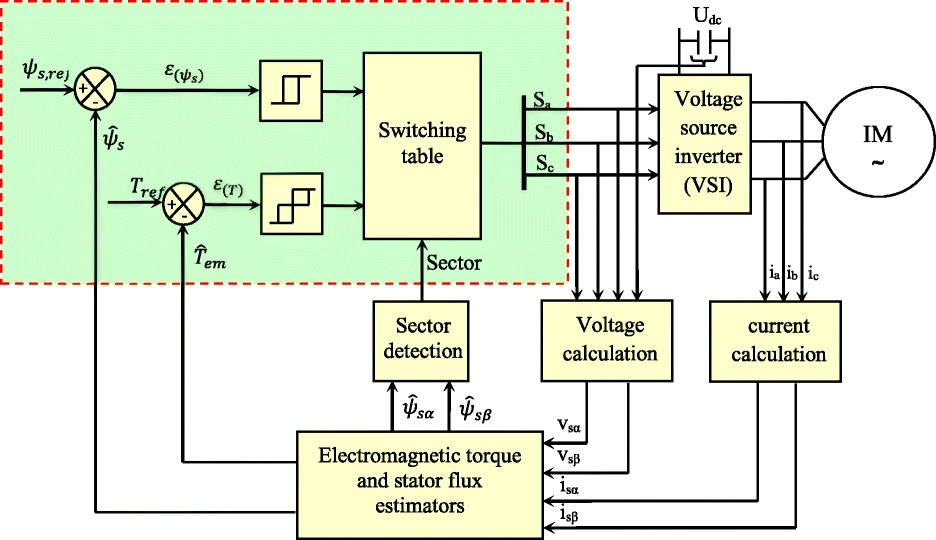
\includegraphics[width=0.8\textwidth]{Figures/dtc_schema.jpg}
	\caption[Direct Torque Control - from~\citet{Quanjli:DTC_schema:2019}.]{Direct Torque Control - from~\citet{Quanjli:DTC_schema:2019}.}
	\label{fig:example_DTC} %chktex 24
\end{figure}
Note that the nature of only switching vectors when the hysteresis is surpassed results in a variable switching frequency as opposed to \gls{foc} that has a fixed switching frequency. Another feature of the \gls{dtc} is that it does not need any modulators, as it directly chooses the voltage vector to be applied.

\gls{dtc} is a very accessible method, with simpler implementation than \gls{foc} a faster dynamic response and low sensitivity to motor parameters, but it falls short in steady state operation with torque and current ripple often bigger than its rival \gls{foc}~\cite{Zhong:DTC_pmsm_dynamics:1997,Niu:DTC_vs_other_DTC_vs_FOC:2016}.



\subsection{Model Predictive Control}
With the increase in computational power, the \gls{mpc} has gained space among the machine controllers as it handles multivariable non-linear cases, is easy to integrate constraints, and has a great dynamic response and integrates constraint managing~\cite{Vazquez:MPC_uses:2014}. The model predictive controller's basic idea is to use a mathematical model of the controlled system to test several control actions and make a prediction about the system response. This prediction is then evaluated by a cost function that can include some soft constraints and the control action with the smaller cost is chosen as optimal.~\citet{Vazquez:MPC_in_power_systems_review:2017:IEEE} classifies the topologies typically used in power converters and drives into continuous set, and finite set, based on the process used to find the optimal control. 

Continuous set is very similar to predictive controllers used on other control fields, it computes a continuous control signal and uses a modulator to generate these voltage vectors. This topology comes with the advantage of fixed switching frequency at the cost of harder implementation and processing power requirements, as it needs an optimization solver. The finite set topology explores the limited control options of power converters to simplify the optimization process. This topology tests a set of the possible control vectors (this set can contain all or part of the possible vectors), and evaluates each of the vectors based on the predictions. While simpler to formulate, this method results in the chosen vector being applied to the full switching period, which results in a higher ripple when compared with a strategy that uses a modulator at the same control frequency. Another property of this strategy is the variable switching frequency, as the same vector can be chosen consecutively. 

To reduce the problem of applying the vector for the full timestep, a subset of finite set topology was presented. It adds time as part of the equation by computing the optimal switching sequence instead of the optimal switching vector, similar to a modulator~\cite{Vazquez:MPC_in_power_systems_review:2017:IEEE}. This allows the controller to choose a set of vectors to be switched in a given sequence with a duration also chosen by the controller.

When applied to \gls{pmsm} the predictive controllers are commonly designed with the dq0 model \Cref{eq:motor_with_inductances_no_derivative}~\cite{Sun:MPC_deadbeat_PMSM:2021}, and may track the currents or the torque to a given reference. The current tracking computational cost tends to be lower as the current optimization can be done offline while tracking torque makes online parameter estimation easier. If the topology is chosen to be continuous, a solver needs to be designed, one of the approaches is to expand the model and cost function into Taylor series approximations, and then use the derivative of the cost function to create a control law~\cite{Errouissi:MPC_taylor_series:2012}. 
% The main issues with developing an \gls{mpc} are to correctly model the system, proper cost function design, and manage computational cost to enable implementation,